\section{Utilizzo dell'Applicazione}
\label{cap:utilizzo}
\subsection{Schermata principale}
All'avvio, la schermata di principale (Figura~\ref{fig:login}) permette di:
\begin{itemize}
    \item Effettuare il login con \textbf{Username} e \textbf{Password}, se già registrati.
    \item Registrare una nuova utenza (cliente o ristoratore).
    \item Accedere come ospite, fornendo delle coordinate geografiche per individuare i ristoranti più vicini.
\end{itemize}

\begin{figure}[H]
    \centering
    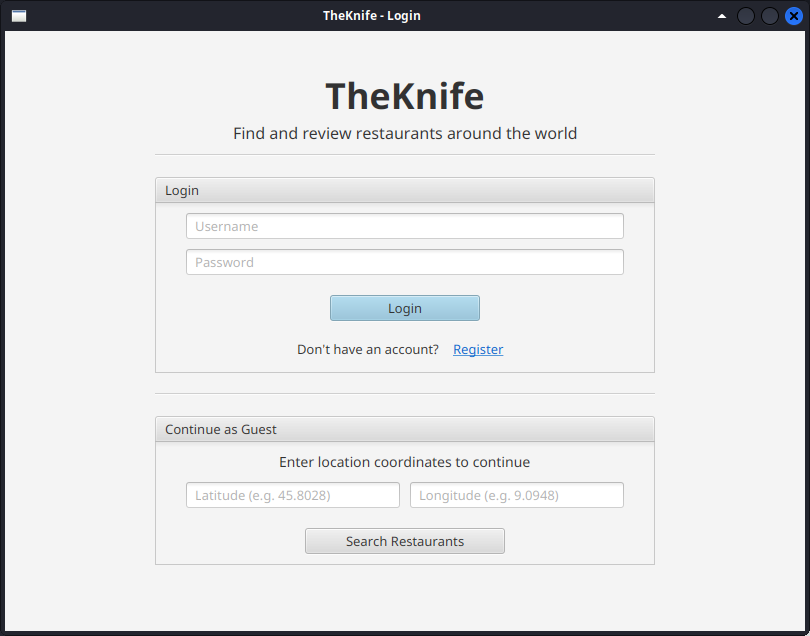
\includegraphics[width=0.8\textwidth]{images/login.png}
    \caption{Schermata principale}
    \label{fig:login}
\end{figure}

\subsection{Registrazione}
Per effettuare la Registrazione premere sul pulsante \emph{register} nella schermata principale (Figura~\ref{fig:registration}).\\
Prosiguire con i seguenti passi:
\begin{enumerate}
    \item Compilare tutti i campi.
    \item Selezionare il tipo di account: \emph{Cliente} o \emph{Ristoratore}.
    \item Confermare tramite email: un link di validazione verrà inviato automaticamente.
\end{enumerate}
\begin{figure}[H]
    \centering
    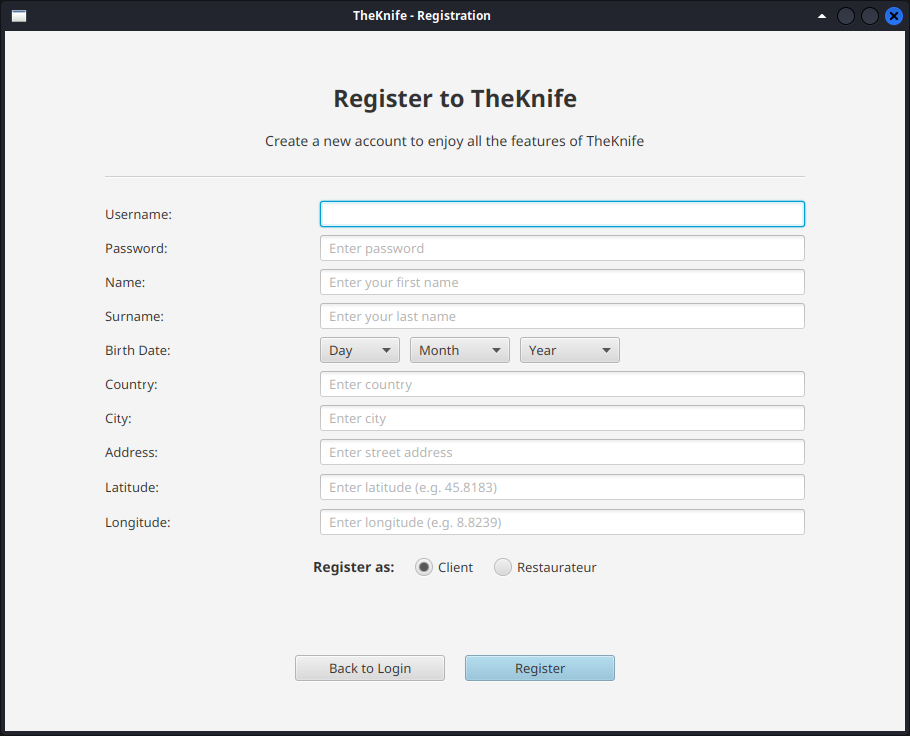
\includegraphics[width=0.8\textwidth]{images/registration.png}
    \caption{Registrazione}
    \label{fig:registration}
\end{figure}
Una volta terminata la registrazione, l'utente potrà effettuare il login con le credenziali scelte.

\subsection{Ricerca e Filtri}
Dopo il login, si accede alla schermata di ricerca (Figura~\ref{fig:search}). È possibile:
\begin{itemize}
    \item Filtrare per tipologia di cucina, fascia di prezzo, consegna a domicilio, prenotazione online, valutazione minima.
    \item Ordinare per distanza, popolarità o voto medio.
    \item Visualizzare un riepilogo sintetico (immagine, nome, voto).
\end{itemize}

\begin{figure}[H]
    \centering
    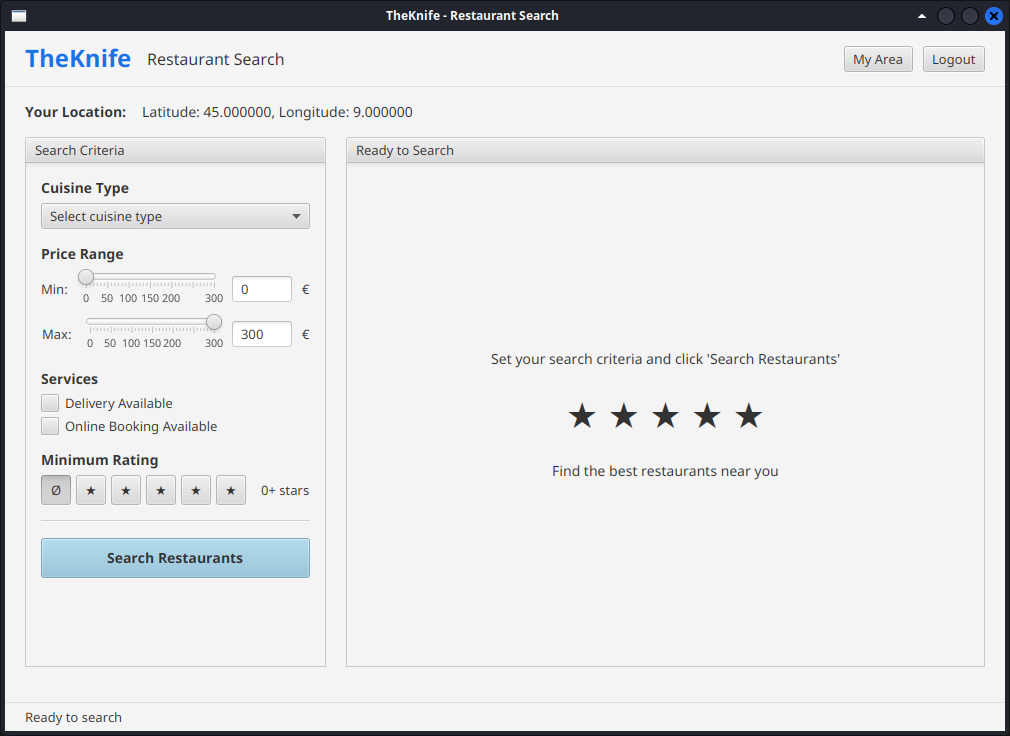
\includegraphics[width=0.8\textwidth]{images/search.png}
    \caption{Schermata di ricerca}
    \label{fig:search}
\end{figure}
Verrano mostrati all'utente i ristoranti più vicini che soddisfino i criteri di ricerca selezionati.

\subsection{Dettaglio ristorante}
Selezionando un ristorante si accede alla pagina di dettaglio (Figura~\ref{fig:restaurant}), che include:
\begin{itemize}
    \item Indirizzo completo
    \item Coordinate geografiche (latitudine e longitudine)
    \item Distanza dall'utente
    \item Rating medio e numero di recensioni
    \item Prezzo medio
    \item Disponibilità di consegna a domicilio e prenotazione online
    \item Recensioni degli utenti
    \item Pulsante per aggiungere ai \emph{Preferiti} (solo utenti registrati).
    \item Pulsante pre creare una nuova recensione (solo utenti registrati).
\end{itemize}

\begin{figure}[H]
    \centering
    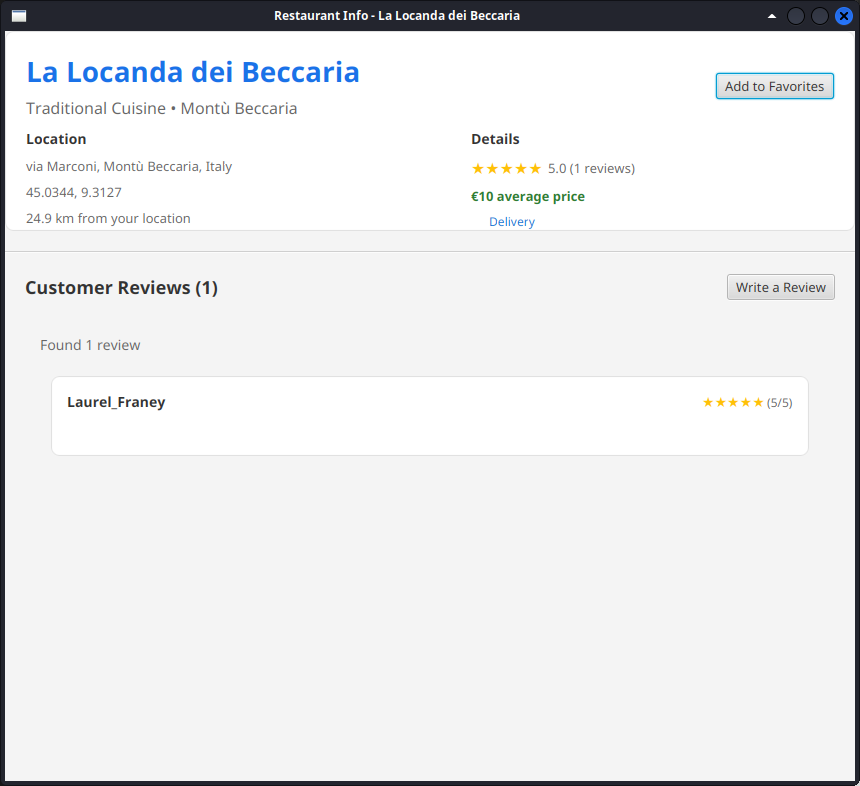
\includegraphics[width=0.8\textwidth]{images/restaurant.png}
    \caption{Pagina di dettaglio del ristorante}
    \label{fig:restaurant}
\end{figure}
